\documentclass[8pt]{beamer}
\usepackage[utf8]{inputenc}
\usepackage{xcolor}
\usepackage{colortbl}
\usepackage{epsfig}
% \usepackage{cancel}
\usepackage{ulem}
% \usepackage{threeparttable} % Joao Pela: 
\usepackage{amsmath}
\usepackage{hyperref}
\usepackage{appendixnumberbeamer}
% \usepackage{feynmp}         % For latex produced Feynman Diagrams

% Rule for feynmp diagrams to be considered graphics
% \DeclareGraphicsRule{*}{mps}{*}{}
% 
% % New compile sequence for feynmp
% \makeatletter
% \def\endfmffile{%
%   \fmfcmd{\p@rcent\space the end.^^J%
%           end.^^J%
%           endinput;}%
%   \if@fmfio
%     \immediate\closeout\@outfmf
%   \fi
%   \ifnum\pdfshellescape=\@ne
%     \immediate\write18{mpost \thefmffile}%
%   \fi}
% \makeatother

\usetheme{Madrid}

\author[J. Pela]{João Pela}
\title[MC VBF QCD]{MC VBF+MET QCD Samples Studies}
\institute[ICL]{Imperial College London}
\date{2014-02-25}

% The log drawn in the upper right corner.
\logo{\includegraphics[height=0.115\paperheight]{img/Logo_CMSICL.png}}

\begin{document}
\setlength{\unitlength}{1mm}

% ###################################################
\begin{frame}
  \titlepage
\end{frame}

% ###################################################
\begin{frame}{Today's presentation}
 
\begin{block}{Topics}
 
\begin{itemize}
  \item 
\end{itemize}
 
\end{block}

\end{frame}

% ###################################################
\begin{frame}{Introduction}


QCD are by far the most frequent processes in collisions at CMS. The elevated cross sections of such processes mean it is normally impossible to generate samples big enough to simulate 
significant amounts of of equivalent luminosity so they can be used in data analysis.

\begin{block}{Methodology}

In order to overcome this problem we generated MC QCD samples with MET plus VBF-like jets.
\begin{itemize}
  \item Real MET (vectorial sum of generator level neutrino $p_T$)
  \item VBF-like jets (AK5 generator level jets)
\end{itemize}

\end{block}

This type of event have a significantly smaller cross section and so to simulate high integrated luminosity samples. 
 
\end{frame}

% ###################################################
\begin{frame}{MC Filter Details}
 
\begin{block}{MC Filter: Vectorial sum of neutrino $E_T$}

  \begin{itemize}
     \item $\sum E_\perp(\vec{\nu}) > 40$ $GeV$
  \end{itemize}

\end{block}

\begin{block}{MC Filter: Dijet Filter}

  \begin{itemize}
    \item Select jets with:
    \begin{itemize}
      \item $p_\perp>20$ $GeV$
      \item $|\eta|<5.0$
    \end{itemize}
    \item From selected jets at least one pair with:
    \begin{itemize}
      \item $m_{jj}>700$ $GeV$
      \item $\Delta\eta>3.2$
    \end{itemize}    
  \end{itemize}

\end{block}

\end{frame}

% ###################################################
\begin{frame}{Testing AM-BDT on QCD I}
 
\begin{block}{How:}

  \begin{itemize}
    \item Some bugs found and fixed and now BDT code is working
    \item Next plots are produced with the following conditions:
    \begin{itemize}
      \item Pass VBF trigger (L1+HLT)
      \item Same point of the prompt selection where BDT was trained. Implies passing vetos, having 2 reconstructed jets, etc.
      \item Pass generator jets cut (same as MC VBF QCD samples)
    \end{itemize}
     item We will use as reference the BDT cut of 0.3 (working point recomended by AM)
  \end{itemize}

\end{block}

\begin{columns}

\column[t]{0.45\linewidth}
\begin{block}{BDT Score $> 0.0$}
 
\centering
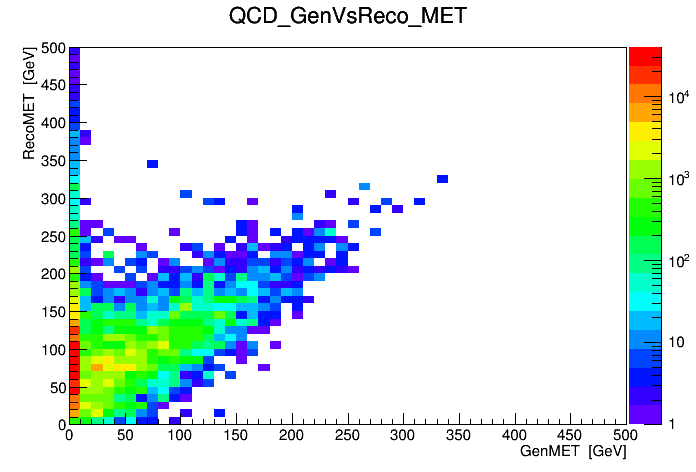
\includegraphics[width=\linewidth]{img/BDT0p0_QCD_GenVsReco_MET.png} 
 
\end{block}

\column[t]{0.45\linewidth}
\begin{block}{BDT Score $> 0.3$}
 
\centering
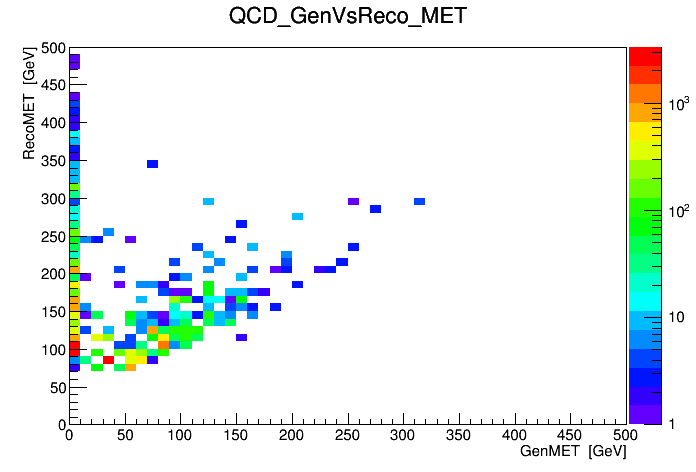
\includegraphics[width=\linewidth]{img/BDT0p3_QCD_GenVsReco_MET.png} 
 
\end{block}

\end{columns}

\end{frame}

% ###################################################
\begin{frame}{Testing AM-BDT on QCD I}
 
\begin{columns}

\column[t]{0.45\linewidth}
\begin{block}{BDT Score $> 0.5$}
 
\centering
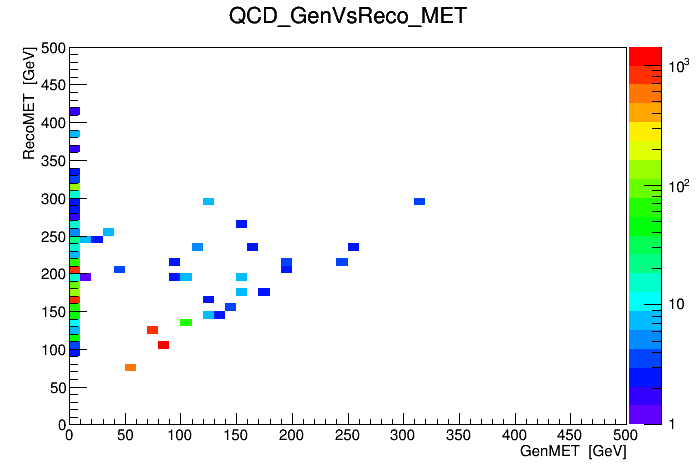
\includegraphics[width=\linewidth]{img/BDT0p5_QCD_GenVsReco_MET.png} 
 
\end{block}

\column[t]{0.45\linewidth}
\begin{block}{BDT Score $> 0.75$}
 
\centering
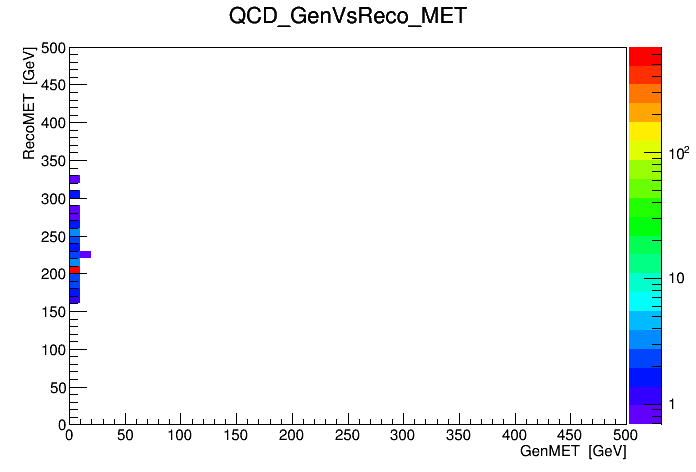
\includegraphics[width=\linewidth]{img/BDT0p75_QCD_GenVsReco_MET.png} 
 
\end{block}

\end{columns} 
 
\end{frame}

% ###################################################
\begin{frame}{Trying $\Delta\phi$ to kill fake QCD I}
 
\begin{block}{How:}

  \begin{itemize}
    \item Next plots are produced with the following conditions:
    \begin{itemize}
      \item Having 2 reconstructed jets (with jets passing prompt selecton conditions).
      \item Pass generator jets cut (same as MC VBF QCD samples)
    \end{itemize}
    \item Since this was just a quick look just used QCD Pt470-600 GeV
  \end{itemize}

\end{block}

\begin{columns}

\column[t]{0.30\linewidth}
\begin{block}{$\Delta\phi<3.0$}
 
\centering
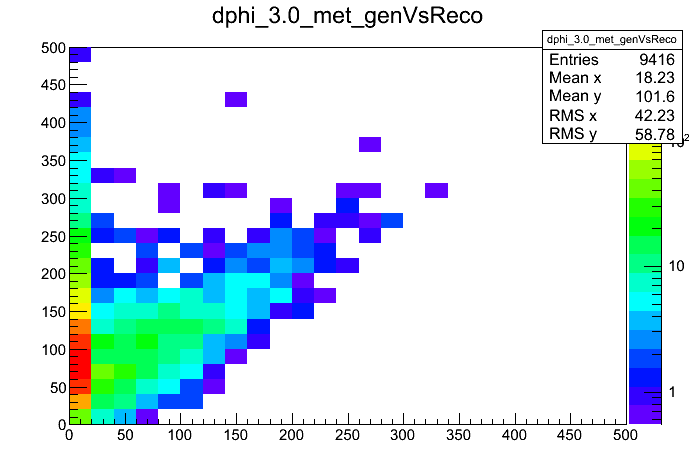
\includegraphics[width=\linewidth]{img/dphi_3p0_met_genVsReco.png} 
 
\end{block}

\column[t]{0.30\linewidth}
\begin{block}{$\Delta\phi<2.5$}
 
\centering
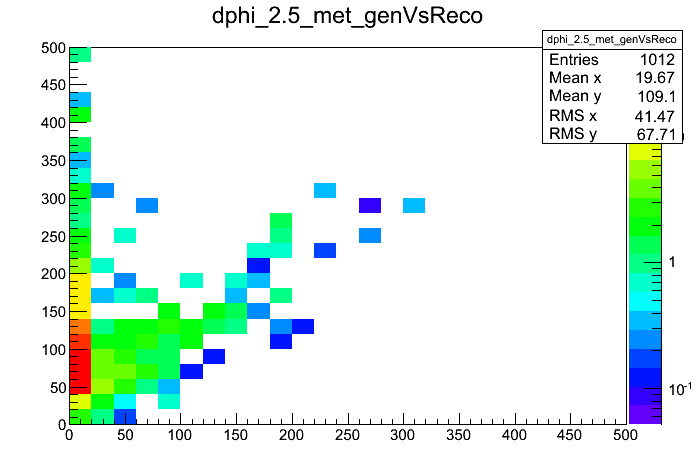
\includegraphics[width=\linewidth]{img/dphi_2p5_met_genVsReco.png} 
 
\end{block}

\column[t]{0.30\linewidth}
\begin{block}{$\Delta\phi<2.0$}
 
\centering
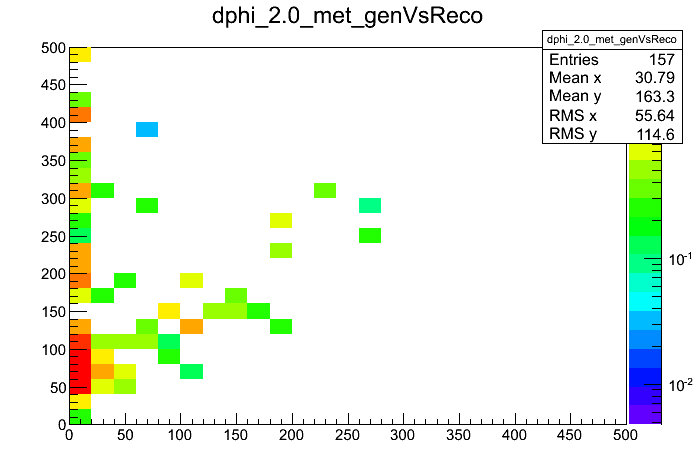
\includegraphics[width=\linewidth]{img/dphi_2p0_met_genVsReco.png} 
 
\end{block}


\end{columns}

\end{frame}

% ###################################################
\begin{frame}{Trying $\Delta\phi$ to kill fake QCD II}

\begin{columns}

\column[t]{0.35\linewidth}
\begin{block}{$\Delta\phi<1.5$}
 
\centering
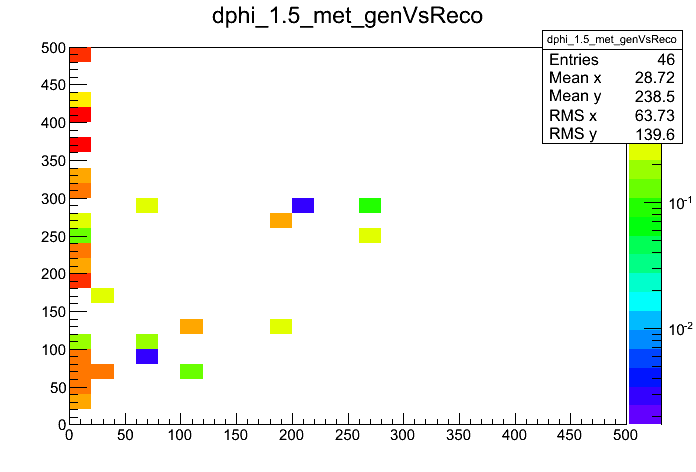
\includegraphics[width=\linewidth]{img/dphi_1p5_met_genVsReco.png} 
 
\end{block}

\begin{block}{$\Delta\phi<1.0$}
 
\centering
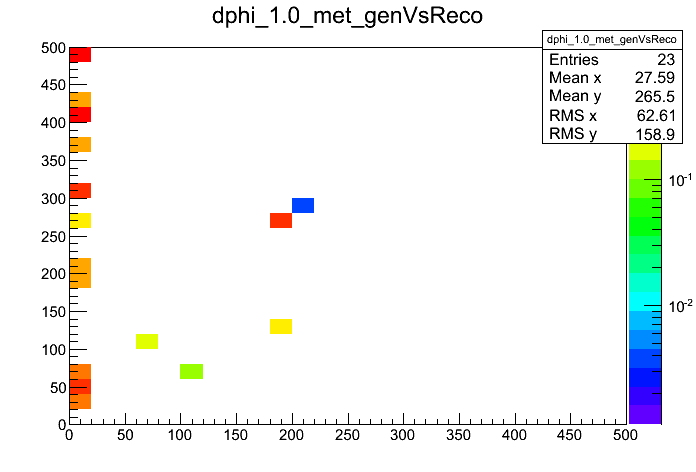
\includegraphics[width=\linewidth]{img/dphi_1p0_met_genVsReco.png} 
 
\end{block}


\column[t]{0.35\linewidth}
\begin{block}{$\Delta\phi<0.5$}
 
\centering
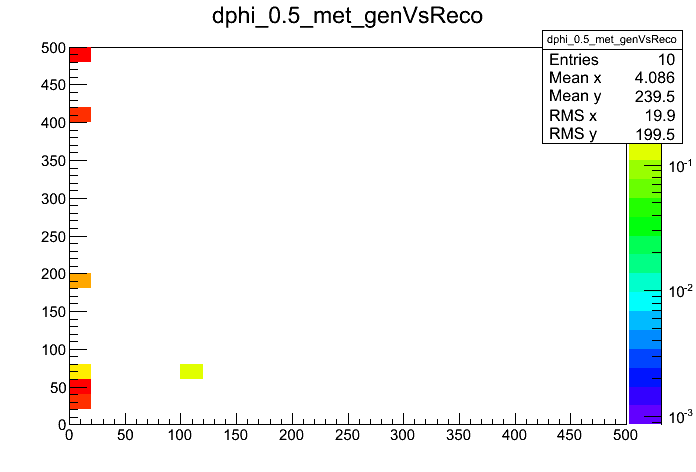
\includegraphics[width=\linewidth]{img/dphi_0p5_met_genVsReco.png} 
 
\end{block}

\begin{block}{$\Delta\phi<0.0$}
 
\centering
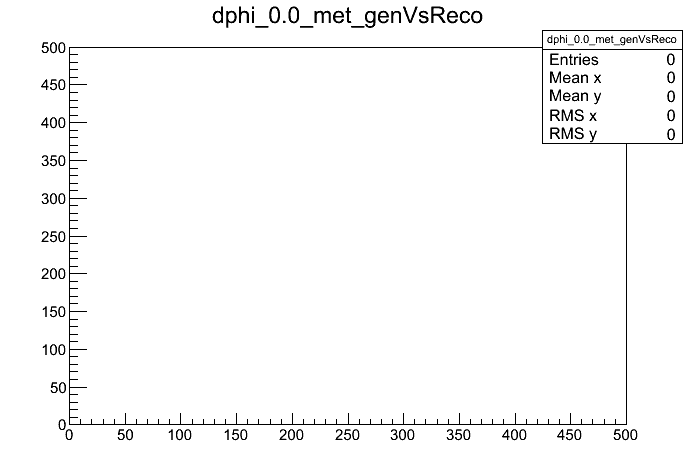
\includegraphics[width=\linewidth]{img/dphi_0p0_met_genVsReco.png} 
 
\end{block}


\end{columns} 
 
\end{frame}










% % ###################################################
% \begin{frame}{Summary and next steps}
%  
% \begin{block}{Summary:}
%  
% \begin{itemize}
%   \item 
% \end{itemize}
% 
% \end{block}
% 
% \begin{block}{Next Steps:}
%  
% \begin{itemize}
%  \item 
% \end{itemize}
%  
% \end{block}
% 
% \end{frame}


% ###################################################
\appendix
% ###################################################
\begin{frame}
 
\begin{block}

\begin{center}Backup Slides\end{center}

\end{block}

\end{frame}

% ###################################################
\begin{frame}{$BDT>0.3$ - Plots by Sample I }

\begin{columns}

\column[t]{0.35\linewidth}
\begin{block}{QCD\_Pt-30to50}
 
\centering
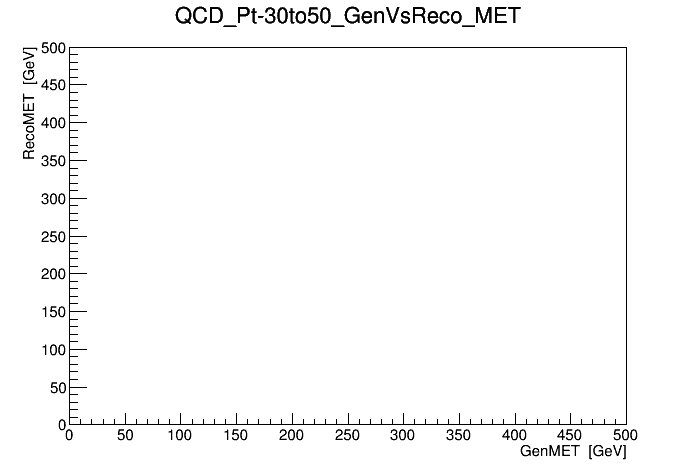
\includegraphics[width=\linewidth]{img/QCD_Pt-30to50_GenVsReco_MET.png} 
 
\end{block}

\begin{block}{QCD\_Pt-80to120}
 
\centering
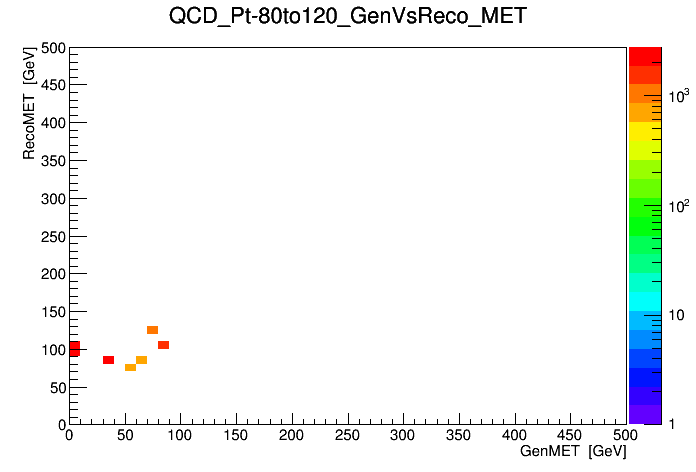
\includegraphics[width=\linewidth]{img/QCD_Pt-80to120_GenVsReco_MET.png} 
 
\end{block}


\column[t]{0.35\linewidth}
\begin{block}{QCD\_Pt-50to80}
 
\centering
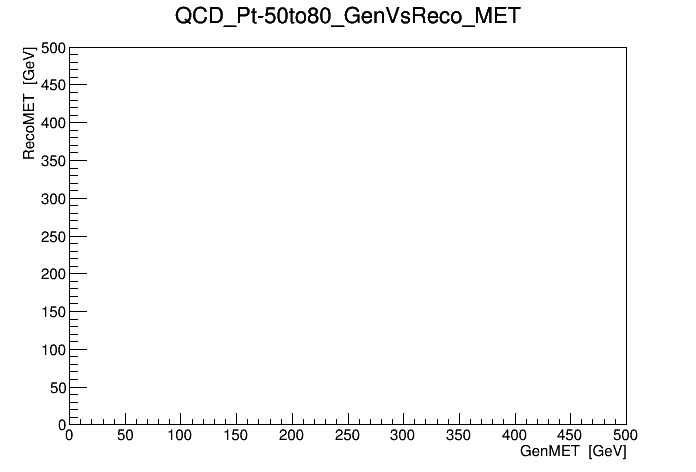
\includegraphics[width=\linewidth]{img/QCD_Pt-50to80_GenVsReco_MET.png} 
 
\end{block}

\begin{block}{QCD\_Pt-120to170}
 
\centering
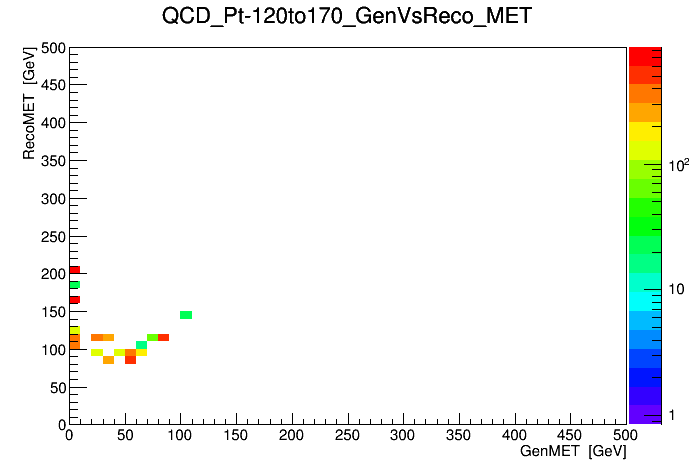
\includegraphics[width=\linewidth]{img/QCD_Pt-120to170_GenVsReco_MET.png} 
 
\end{block}


\end{columns} 
 
\end{frame}

% ###################################################
\begin{frame}{$BDT>0.3$ - Plots by Sample II}

\begin{columns}

\column[t]{0.35\linewidth}
\begin{block}{QCD\_Pt-170to300}
 
\centering
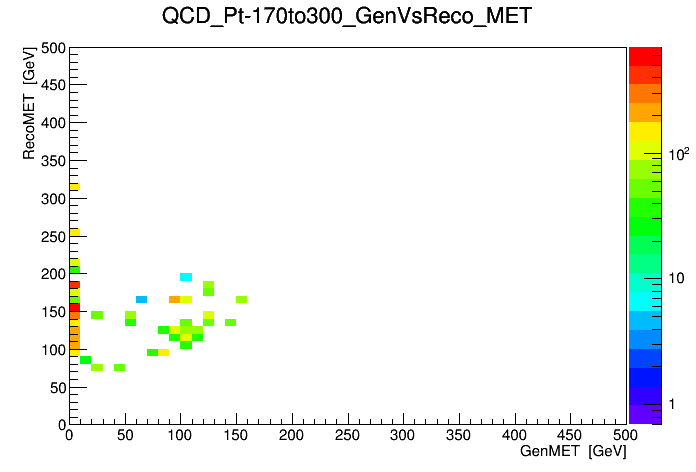
\includegraphics[width=\linewidth]{img/QCD_Pt-170to300_GenVsReco_MET.png} 
 
\end{block}

\begin{block}{QCD\_Pt-470to600}
 
\centering
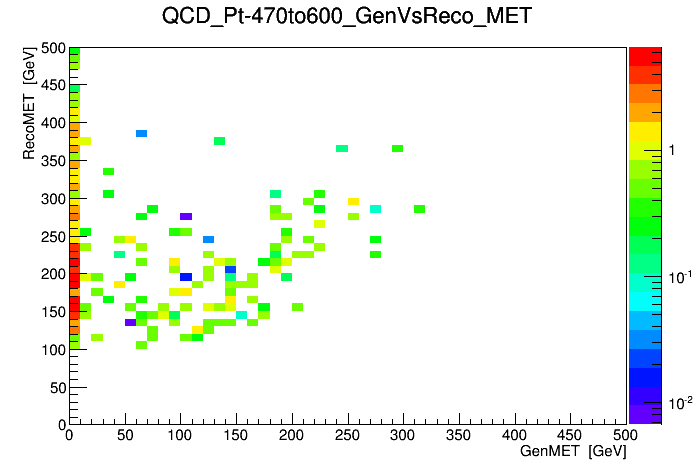
\includegraphics[width=\linewidth]{img/QCD_Pt-470to600_GenVsReco_MET.png} 
 
\end{block}


\column[t]{0.35\linewidth}
\begin{block}{QCD\_Pt-300to470}
 
\centering
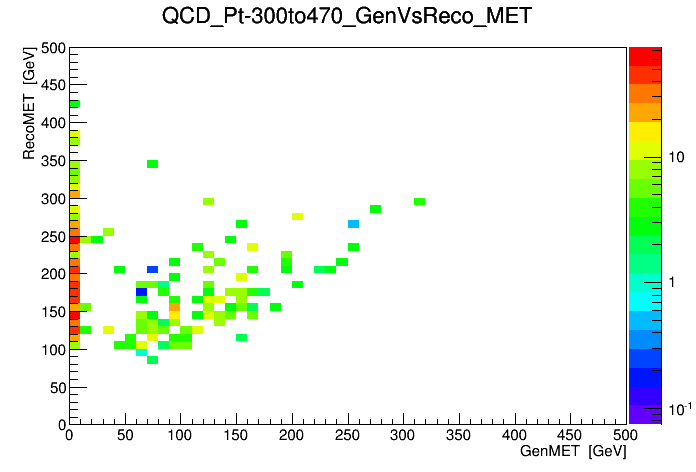
\includegraphics[width=\linewidth]{img/QCD_Pt-300to470_GenVsReco_MET.png} 
 
\end{block}

\begin{block}{QCD\_Pt-600to800}
 
\centering
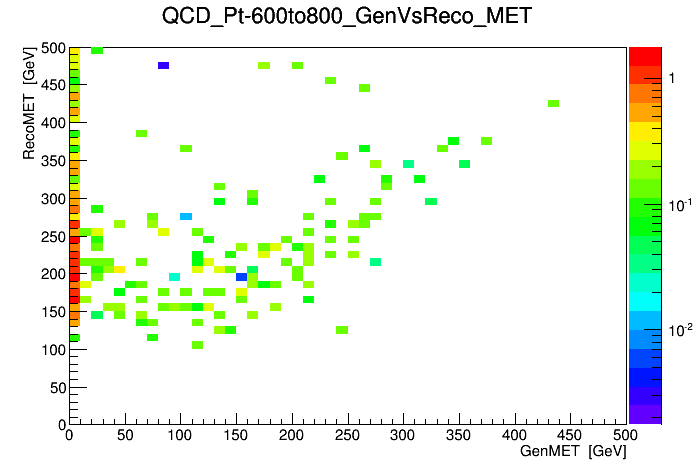
\includegraphics[width=\linewidth]{img/QCD_Pt-600to800_GenVsReco_MET.png} 
 
\end{block}


\end{columns} 
 
\end{frame}

% ###################################################
\begin{frame}{$BDT>0.3$ - Plots by Sample III}

\begin{columns}

\column[t]{0.35\linewidth}
\begin{block}{QCD\_Pt-800to1000}
 
\centering
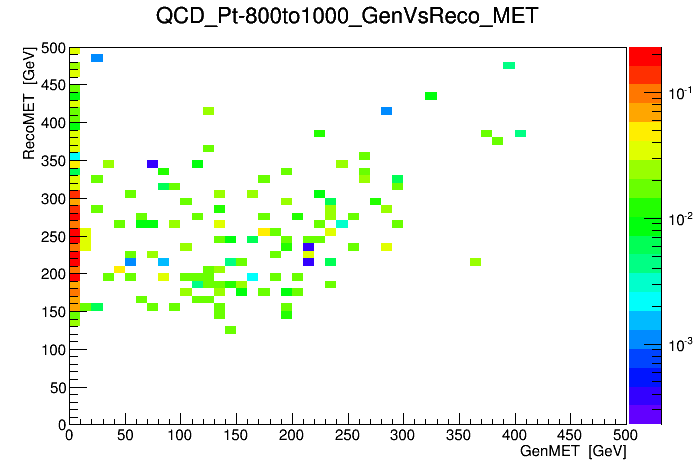
\includegraphics[width=\linewidth]{img/QCD_Pt-800to1000_GenVsReco_MET.png} 
 
\end{block}

\begin{block}{QCD\_Pt-1400to1800}
 
\centering
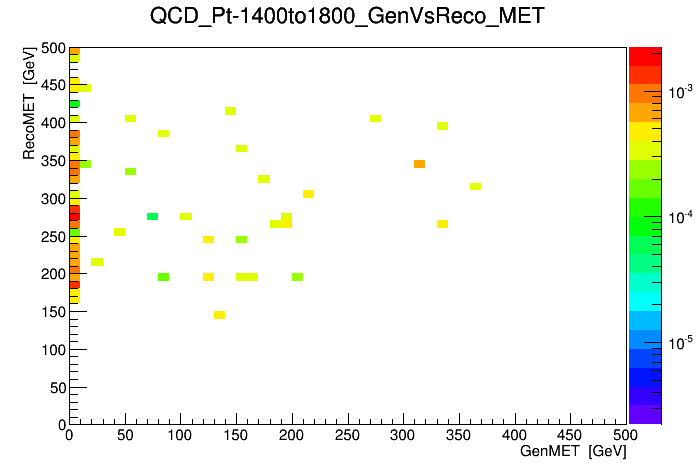
\includegraphics[width=\linewidth]{img/QCD_Pt-1400to1800_GenVsReco_MET.png} 
 
\end{block}


\column[t]{0.35\linewidth}
\begin{block}{QCD\_Pt-1000to1400}
 
\centering
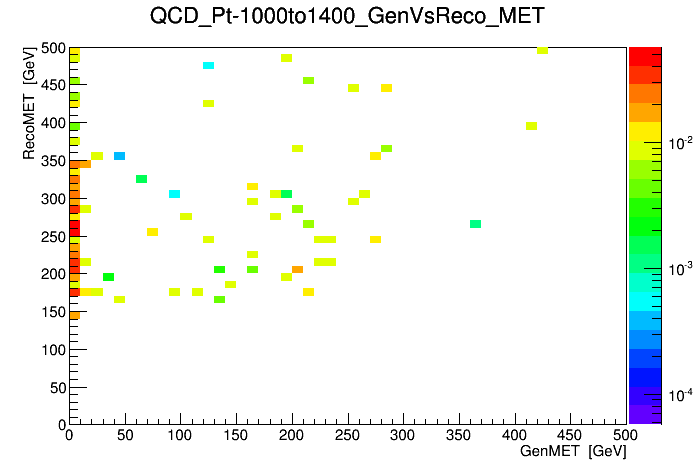
\includegraphics[width=\linewidth]{img/QCD_Pt-1000to1400_GenVsReco_MET.png} 
 
\end{block}

\begin{block}{QCD\_Pt-1800}
 
\centering
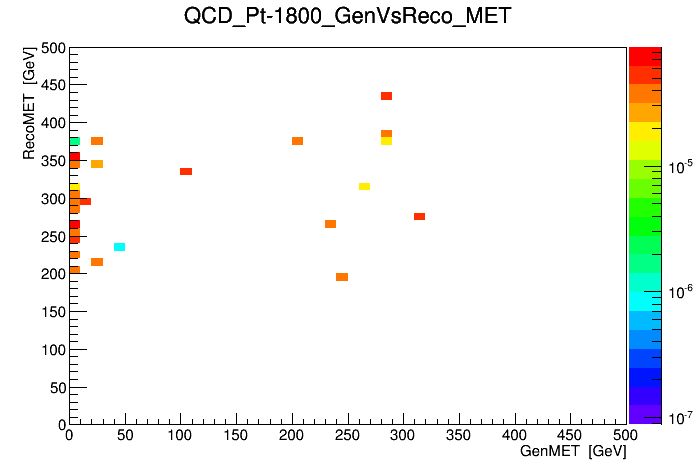
\includegraphics[width=\linewidth]{img/QCD_Pt-1800_GenVsReco_MET.png} 
 
\end{block}

\end{columns} 
 
\end{frame}

% ###################################################
\begin{frame}{$BDT>0.3$ - Plots by Sample III}

\begin{columns}

\column[t]{0.35\linewidth}
\begin{block}{GJets-HT-200To400}
 
\centering
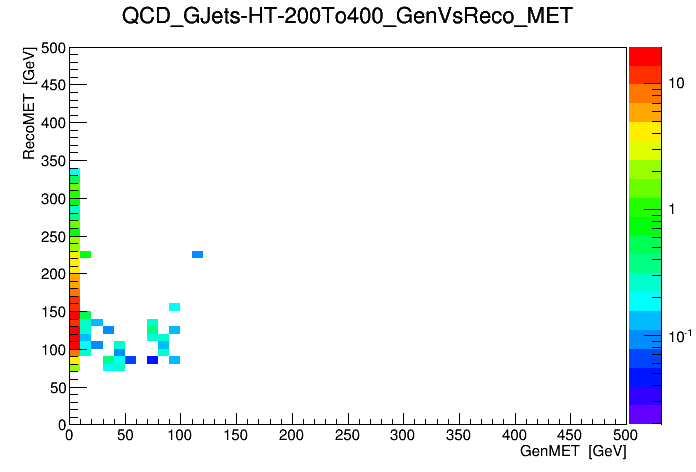
\includegraphics[width=\linewidth]{img/QCD_GJets-HT-200To400_GenVsReco_MET.png} 
 
\end{block}

\column[t]{0.35\linewidth}
\begin{block}{GJets-HT-400ToInf}
 
\centering
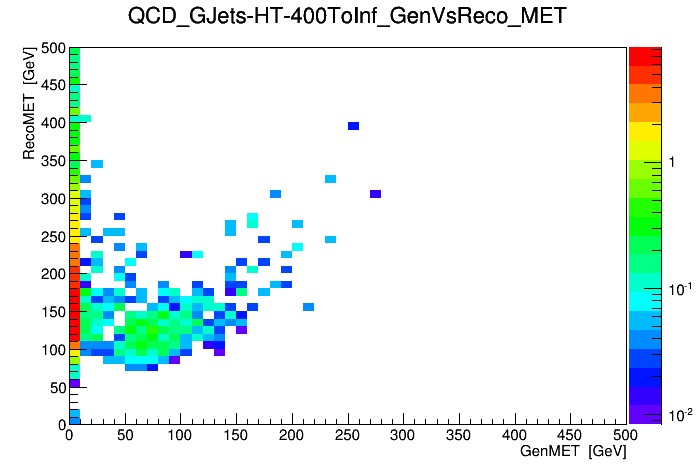
\includegraphics[width=\linewidth]{img/QCD_GJets-HT-400ToInf_GenVsReco_MET.png} 
 
\end{block}

\end{columns} 
 
\end{frame}

\end{document}